In this report, we describe the program we created to simulate a system of conveyor belts that transport luggage items.

The system could potentially be used as a tool for modelling for example a luggage system at an airport. However, we have decided to make our application more like a game, since a real simulation system would be very difficult to make and furthermore require specialized domain knowledge about the system to simulate.

Before we started working on the project, we created a mock-up, as shown in Figure~\ref{fig:mockup}.

\begin{figure}
  \begin{center}
    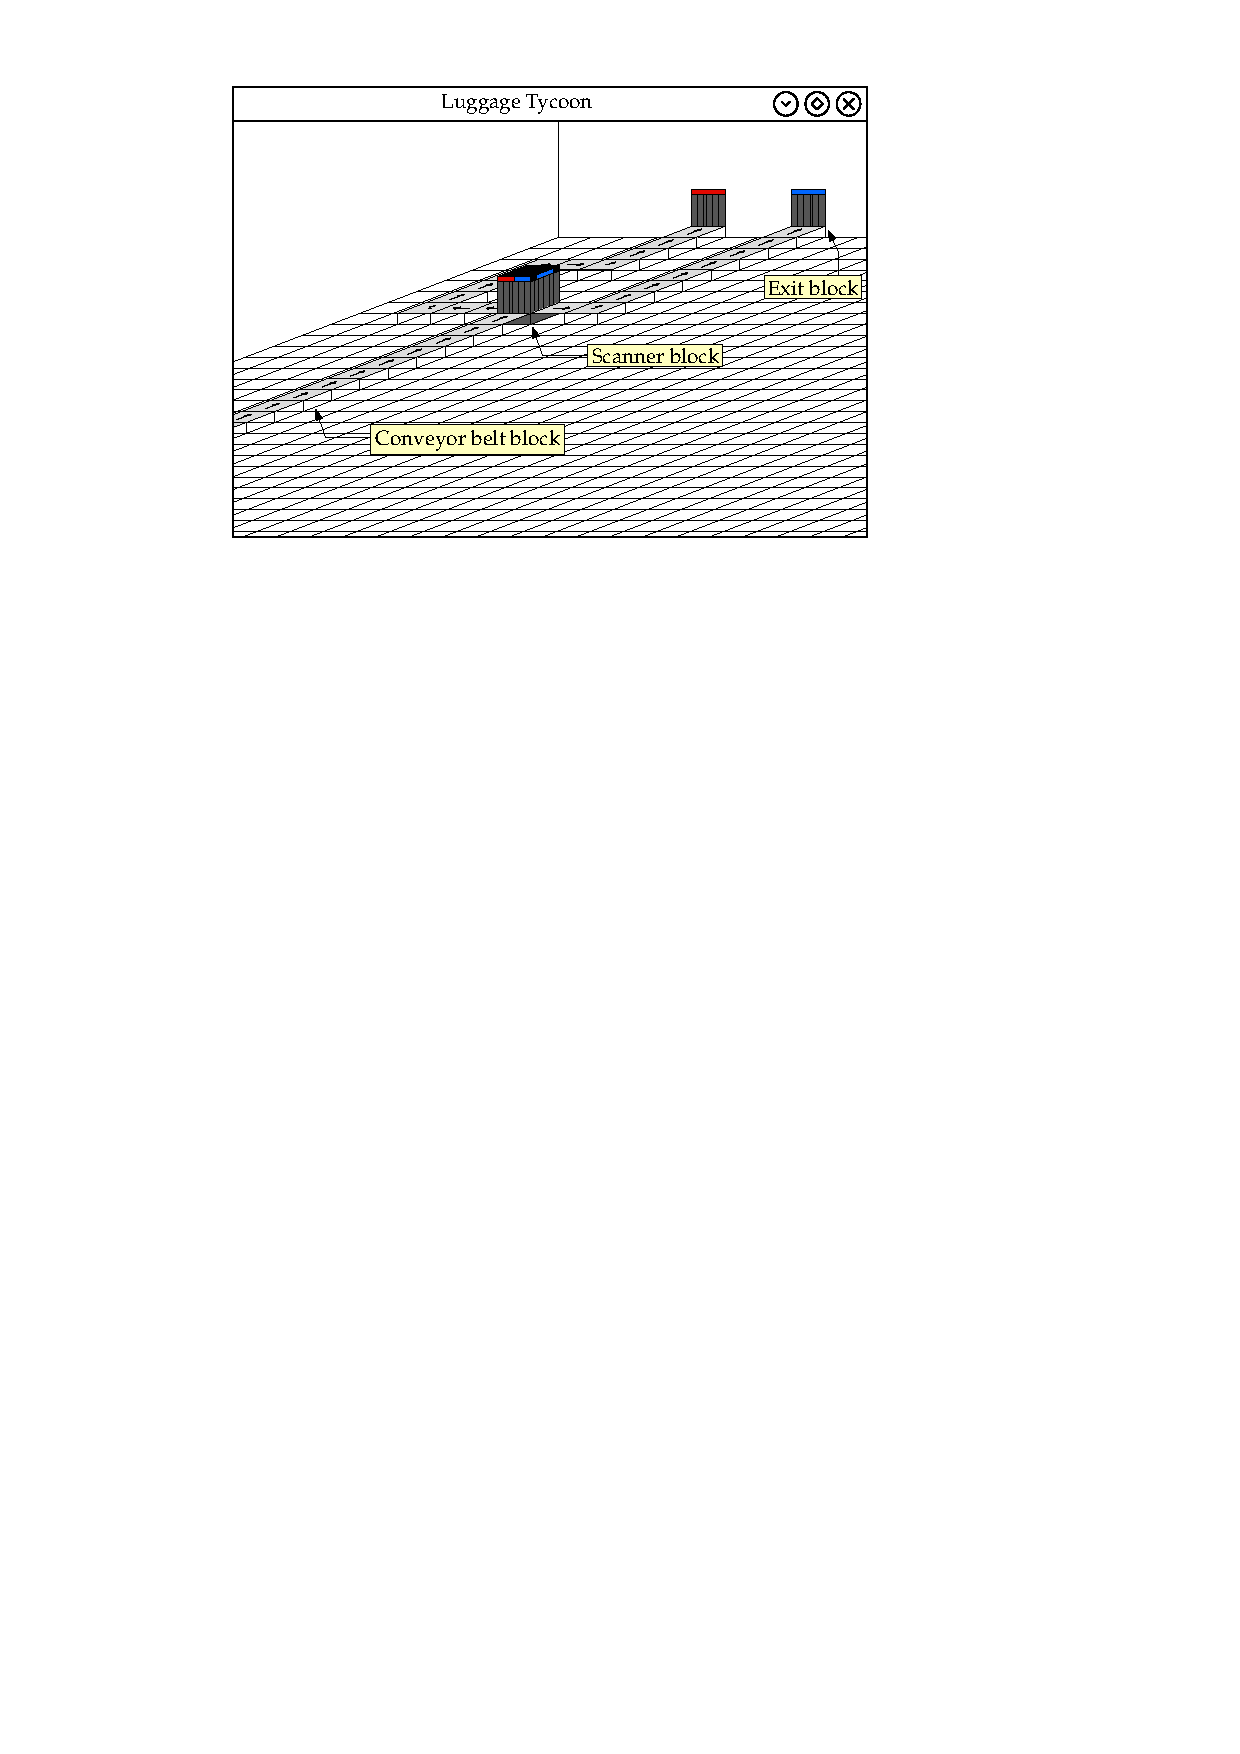
\includegraphics{mockup}
    \caption{A mock-up of the program we wanted to create.}
    \label{fig:mockup}
  \end{center}
\end{figure}
